% !TEX root = ../../../under-spec-z.tex

\section{Introduction} % (fold)
\label{sec:introduction}

    \subsection{Formatting} % (fold)
    \label{ssub:formatting}

        This paper consists of translated sections from \cite{Toen:2005wxa} as well as the author's own writing.
        The general layout and order tries to follow that of the original paper as much as possible, including section numbering and naming.

        Longer sections of translated text will be boxed, left aligned, sans serif, and ended with a small black square ($\blacksquare$).
        At the start of such sections there will also be a reference to the location of the source text.
        Shorter `quotations' will simply be in italics and referenced afterwards.
        Theorems (and definitions) that have been translated will not be boxed off or in quotes, but there will be a reference to the original theorem (or definition) after the theorem (or definition) number.
        Hopefully it will be largely self-explanatory, but here are a few guidelines that the author has tried to adhere to:
        \begin{itemize}
            \item Usually they will be given as a section and a paragraph, e.g. (\S1\,\P2), where the paragraphs are counted by looking at indentations.
            \item Negative paragraph numbers indicate counting from the end of the section (as given), with the last paragraph being the -1st.
                For example, (\S2.1\,\P-2) would indicate the penultimate paragraph of section 2.1.
                (Luckily there are no subsubsections, so we don't have to worry about things getting any more complex.)
        \end{itemize}


        Sometimes a section that we wish to translate will contain some reference to a theorem or definition in the original paper, and this might have a different numbering in \emph{this} paper.
        Because of this, all such references (e.g. \emph{voir définition 2.12}) from the original will be suitably replaced with numbering relevant to \emph{this} paper (e.g. \emph{voir \elide (\cref{le:yoneda-lemma})}).

        If there are any references to a certain section or paragraph without specifying from which paper, then they are to \cite{Toen:2005wxa}.
        Similarly, if any lemma (or theorem) is stated without a proof then a proof can be found in the referenced lemma (or theorem) in \cite{Toen:2005wxa}.

        Finally, all footnotes, in translated sections or not, are by the author and \emph{not} from \cite{Toen:2005wxa}.


    \subsubsection{Conventions} % (fold)
    \label{ssub:conventions}

        We retain the following conventions from \cite{Toen:2005wxa}:
        \begin{translation}{1}{-2}
            All the monoids and monoidal categories considered will be unital and associative, and all modules over a monoid will be unital.
            We will ignore all set-theoretic problems to do with the choice of universe; the reader can consult \cite{Toen:2005er,Toen:2008wy} to find a method to resolve them.
        \end{translation}

        We also impose the following conventions ourselves, which are always assumed (unless otherwise stated):
        \begin{itemize}
            \item all algebras and rings are unital and associative;
            \item $k$ is an algebraically closed field;
            \item $0\in\nn$;
            \item for a ring $R$ we write $R^\times$ to mean the group of multiplicative units in $R$;
            \item $\GG_m=k^\times=k\setminus\{0\}$;
            \item for $n\in\nn\setminus\{0\}$ we write $\mu_n$ to mean the cyclic group of order $n$;
            \item given a category $\ccat$ we write $x\in\ccat$ to mean $x\in\mathrm{ob}(\ccat)$;
            \item `presheaf' means a $\Set$-valued presheaf.
        \end{itemize}
        We usually use `functor' to mean `covariant functor'.
        % It is not a strict convention, but we tend to think of functors as being covariant (and hence contravariant functors are functors from the opposite category).
        % This is not a universal view though, and some papers don't adopt this tendency, but the context should always make it clear how we are thinking about functors.

    % subsubsection conventions (end)


    % !TEX root = ../../../under-spec-z.tex

\subsection{Overview} % (fold)
\label{sub:overview}

    In this paper we will summarise some of the results of \cite{Toen:2005wxa}, providing background definitions along the way, as well as filling in some of the proofs that are omitted or only sketched.
    All of the pictures, as well as \cref{sub:background_knowledge,sec:further_applications}, are entirely original and aim to complement the main results (though the pictures are \emph{not} to be taken too literally -- they often illustrate simple cases, such as when $\ccat=\Op{T}$).
    There are also explanations of motivation (e.g. \cref{sub:under_}) and historical notes (e.g. \cref{sub:the_riemann_hypothesis}) that are original.
    This is why this paper is subtitled `\emph{a readers' guide}', and not simply `\emph{a translation}'.

    The results of \cite{Toen:2005wxa} are many, and we will not have time to cover most of the later sections;  we will focus largely on the first three\footnote{
        Not including the introduction, so sections 2 (\emph{Géométrie algébrique relative}), 3 (\emph{Trois exemples de géométries relatives}), and 4 (\emph{Quelques exemples de schémas au-dessous de $\spec\zz$}).
    } sections.
    Because of this, for us, the introduction of \cite{Toen:2005wxa} summarises the purpose of the paper better than the abstract.

    \vspace{-1em}

    \begin{translation}{1}{1}
        The aim of this paper is to construct several categories of \emph{schemes} that are defined over bases found \emph{under $\spec\zz$}.
        Of course, since $\zz$ is the initial object in the category of commutative rings, it is vital to leave the usual framework of rings and permit the use of more general objects, but only objects that  resemble commutative rings enough such that the notion of a scheme can still be defined.
        Our approach to this problem is based on the theory of relative algebraic geometry, largely inspired by \cite{Hakim:XPnOZC1P}.
        It comes from remarking that a commutative ring is nothing but a commutative monoid in the monoidal category of $\zz$-modules, and that, in general, for a symmetric monoidal category $\smc$, the commutative monoids in $\ccat$ can be thought of as models for the \emph{affine schemes relative to $\ccat$}.
        It is remarkable that such a general (simplistic, even) approach allows us to actually define the notion of schemes, and moreover in a functorial way in $\ccat$.
        So, in choosing $\ccat$ equipped with a sensible symmetric monoidal functor $\ccat\to\modc{\zz}$, we find a notion of schemes relative to $\ccat$ and a base-change functor to $\zz$-schemes, and thus a notion of schemes under $\spec\zz$.
        % In this paper we show how this approach, as well as its \ghl{homotopic generalisation where $\ccat$ is also equipped with a Quillen model structure}, allows us to define five categories of schemes found under $\spec\zz$.
    \end{translation}

% In this translation we mainly focus on section 2 (\emph{Relative algebraic geometry}), about which the introduction has the following to say.

% \begin{translation}{1}{2--5}
%     % The general ideas of relative algebraic geometry date back to \cite{Hakim:XPnOZC1P}, where \ghl{relative schemes over a ringed topos} are defined.
%     % In \cite{Deligne:2007hm} the case of schemes over a \ghl{tannakian category} is also considered.
%     The theory of relative  algebraic geometry that we present here is largely inspired by [\cite{Hakim:XPnOZC1P,Deligne:2007hm}], but considering categories over bases that aren't abelian, nor even additive, appears to be a novelty.
%     \\\\
%     Consider a symmetric monoidal category\footnote{
%         \cref{df:smc}
%     } $\smc$ that we also suppose to be complete, cocomplete, and closed\footnote{
%         Such a category is now often called a \emph{cosmos} (\cref{df:cosmos}).
%     } (i.e. possessing an internal $\Hom$ functor relative to the $\otimes$ monoidal structure).
%     It is well known\footnote{
%         Monoids, modules, and $\comm{\ccat}$ are all defined in \cref{ssub:preliminary_definitions}.
%         The change of base functor is discussed at length in \cref{ssub:change_of_base_for_modules_over_a_monoid}.
%     } that we have: the notion of a monoid in $\ccat$; for such a monoid $A$, the notion of a module; and for a morphism of monoids $A\to B$, a base-change functor $\blank\otimes_A B$ from $A$-modules to $B$-modules (see \cite{Saavedra:1972tn}).
%     In particular there exists the notion of commutative monoids (associative and unital) in $\ccat$, and they form a category that we call $\comm{\ccat}$.
%     We formally define the category of affine schemes relative to $\ccat$ by $\aff{\ccat}=\op{\comm{\ccat}}$.
%     \\\\
%     All of this is, for the moment, completely formal, but it produces a few miracles:
%     \begin{itemize}
%         \item There exists a natural Grothendieck topology on $\aff{\ccat}$ called the {\emph{flat topology}} \elide\footnote{
%             \cref{df:fpqc-topology,df:fpqc-zariski-covers}
%         }.
%         % The covering families $\{X_i\to X\}$ for this topology correspond to the \ghl{finite families of morphisms} $\{A\to A_i\}$ in $\comm{\ccat}$ such that the base-change functor \ghl{on} the category of modules
%         % $$\prod_i\left(\blank\otimes_A A_i\right): \modc{A} \longrightarrow \prod_i\left(\modc{A_i}\right)$$
%         % is exact and conservative.
        
%         \item The flat topology on $\aff{\ccat}$ so defined is subcanonical (i.e. representable presheaves are sheaves).

%         \item There exists the notion of \emph{Zariski open} in $\aff{\ccat}$ \elide\footnote{
%             \cref{df:zariski-open-morphism}
%         }.
%         % , and they are by definition the morphisms $f\colon X\to Y$ for which the corresponding morphism \mbox{$A\to B$} in $\comm{\ccat}$ satisfies the following three conditions:
%         % \begin{enumerate}
%         %     \item \textit{$f$ is a monomorphism:} for all $A'\in\comm{\ccat}$ the \ghl{induced} morphism $\Hom(B,A')\to\Hom(A,A')$ is injective;
            
%         %     \item \textit{$f$ is \ghl{flat}:} the base-change functor
%         %     $$(\blank\otimes_A B) \colon \modc{A} \longrightarrow \modc{B}$$
%         %     is exact;

%         %     \item \textit{$f$ is a finite presentation:} for all filtered diagrams of objects $C_i\in A/\comm{\ccat}$, the natural morphism
%         %     $$\colim\Hom_{A/\comm{\ccat}}(B,C_i) \longrightarrow \Hom_{A/\comm{\ccat}}(B,\colim C_i)$$
%         %     is bijective.
%         % \end{enumerate}

%         \item The notion of Zariski open extends naturally to general morphisms between sheaves (see \elide(\cref{df:zariski-open-sheaves})).

%         \item The Zariski-open morphisms are stable under composition, isomorphism\footnote{
%             That is, composition with an arbitrary isomorphism.
%         }, and change of base.

%         \item The Zariski-open morphisms give rise to a notion of a Zariski topology, and this is again subcanonical.
%     \end{itemize}
    
%     The above properties are all that we need to define a category of schemes relative to $\smc$.
%     Indeed, a relative scheme is by definition a sheaf on the site $\aff{\ccat}$, endowed with the Zariski topology, and possessing a Zariski-open cover by affine schemes (see \elide(\cref{df:relative-scheme})).
%     The categories of schemes thus obtained is denoted $\sch{\ccat}$.
%     It is a full subcategory, stable under pullbacks and disjoint unions, of the category of sheaves on $\aff{\ccat}$.
%     Further it contains a full subcategory of affine schemes, that are exactly the representable sheaves, and is naturally equivalent to the category $\comm{\ccat}$, opposite to the category of commutative monoids in $\ccat$ (see \elide(\cref{sub:the_faithfully_flat_topology})).
%     Finally, the purely categorical nature of the construction makes the category $\sch{\ccat}$ functorial in $\ccat$, at the very least for left symmetric-monoidal adjoints $\smc\to\smd$ satisfying certain (easy to verify in practice) conditions (see \elide(\cref{sub:changes_of_bases})).
% \end{translation}

% subsection overview (end)



    % !TEX root = ../../../under-spec-z.tex

\subsection{Background knowledge} % (fold)
\label{sub:background_knowledge}

    This section acts as a prelude to \cite{Toen:2005wxa}, containing a few motivating examples and prerequisite definitions and lemmas.
    Before diving straight into the abstract definitions, we give an example of why we might think to try a category-theoretic approach to algebraic geometry.

    \subsubsection{Motivating example} % (fold)
    \label{ssub:motivating_example}

        Let $A$ be a finitely-generated commutative $k$-algebra.
        Then we can write
        \begin{equation*}
            A=\frac{k[x_1,\ldots,x_n]}{(f_1,\ldots,f_m)}
        \end{equation*}
        for some $m,n\in\nn$ and $f_i\in k[x_1,\ldots,x_n]$.
        If $B$ is another commutative $k$-algebra (not necessarily finitely generated) then the collection of algebra morphisms $A\to B$ is in bijection with points of $B^n$ that vanish on all of the $f_i$, since a morphism is determined entirely by where it sends each of the $x_i$ whilst satisfying $0\mapsto0$.
        So, letting $\commk$ denote the category of commutative $k$-algebras,
        \begin{equation}\label{eq:link-between-hom-and-varieties}
            \Hom_{\commk}(A,B)\cong\{b\in B^n \mid f_1(b)=\ldots=f_m(b)=0\}
        \end{equation}
        where, as usual, we evaluate $f_i(b)$ inside $B$.

        \Cref{eq:link-between-hom-and-varieties} implies that we should maybe think of $\Hom(A,B)$ as some variety inside $B^n$ determined by $A$, for general $A,B\in\commk$, and so we might be able to recover a lot of algebraic geometry from studying these $\Hom(A,B)$.
        In fact, thinking of $\Hom(A,\blank)$ as a functor $\commk\to\Set$ which takes an algebra $B$ to a \emph{variety} (a set of points) inside $B^n$, we are led to the more general idea of studying \emph{all} functors $\commk\to\Set$, and calling such functors \emph{spaces}.

        Before formalising this, we first recall a few things from category theory.
        
        \begin{definition}[Presheaves]\label{df:presheaves}
            Let $\ccat$ be a category.
            The category of \emph{presheaves on $\ccat$} is defined as the functor category $\PShv(\ccat)=\Fun(\op{\ccat},\Set)$, whose objects are (covariant) functors $\op{\ccat}\to\Set$ and morphisms are natural transformations $F\nt G$ between such functors.
        \end{definition}

        % \begin{figure}[h]
        %     \centering
        %     \frame{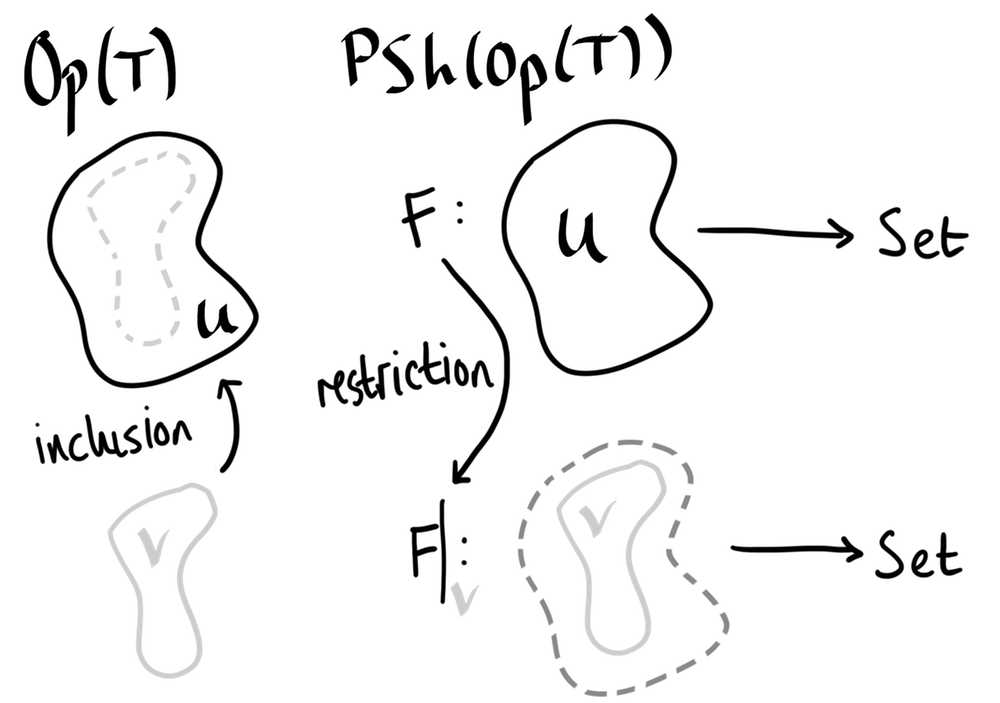
\includegraphics[width=.6\textwidth]{images/presheaves.png}}
        %     \caption{Presheaves on $\Op{T}$ (see paragraph after \cref{df:pullbacks}) -- inclusion of open sets corresponds to restriction of presheaves}
        %     \label{fg:presheaves}
        % \end{figure}

        \begin{figure}[h]
            \centering
            \frame{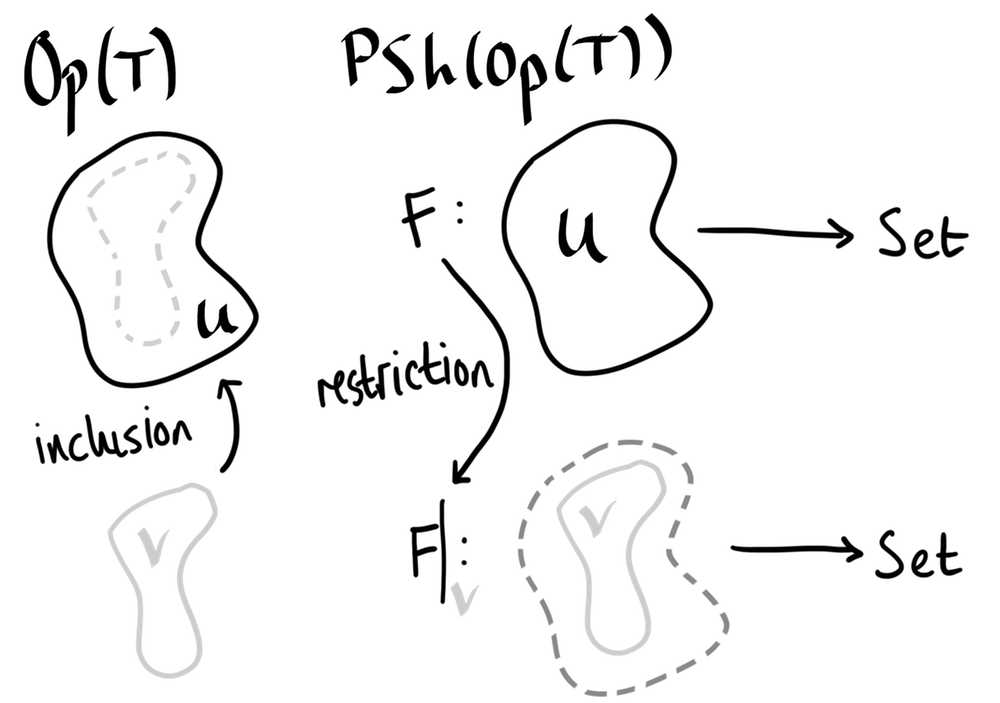
\includegraphics[width=.63\textwidth]{images/presheaves.png}}
            \caption{Presheaves on $\Op{T}$ (see paragraph after \cref{df:pullbacks}) -- inclusion of open sets corresponds to restriction of presheaves}\label{fg:presheaves}
        \end{figure}

        \begin{lemma}[Yoneda lemma]\label{le:yoneda-lemma}
            Let $\ccat$ be a locally small category\footnote{
                That is, the hom-sets $\Hom(A,B)$ are actual sets for all $A,B\in\ccat$.
            }.
            Define the \emph{downwards Yoneda functor}\footnote{
                This is not at all common terminology.
                It is often called the \emph{contravariant Yoneda functor}: it maps an object $A\in\ccat$ to the \emph{contravariant} functor $\Hom_\ccat(\blank,A)\colon\ccat\to\Set$.
                But the functor $\ccat\to\PShv(\ccat)$ itself is \emph{covariant}, so we use `downwards' to avoid confusion.
                The dual `covariant' (\emph{upwards}, in our terminology) functor is $Y^{(\blank)}\colon\op{\ccat}\to\Fun(\ccat,\Set)$ given by $\spec A\mapsto Y^A=\Hom_\ccat(A,\blank)$, where we write $\spec A\in\op{\ccat}$ to be the object corresponding to $A\in\ccat$.
                Then the statement $\Hom_{\Fun(\ccat,\Set)}(Y^A,G)\cong G(A)$ holds.
            } by
            \begin{align*}
                Y_{(\blank)}\colon&\ccat\to\PShv(\ccat)\\
                &A\mapsto \Hom_\ccat(\blank, A),
            \end{align*}
            which is well defined, since $\Hom(\blank, A)\colon\op{\ccat}\to\Set$ covariantly.
            Then, for any $A\in\ccat$ and $F\in\PShv(\ccat)$,
            \begin{equation}
                \Hom_{\PShv(\ccat)}(Y_A,F) \cong F(A)
            \end{equation}
            via the canonical restriction map.
            Further, $Y$ is fully faithful.
        \end{lemma}

        \begin{proof}
            See \cite[\S III.2, p.59--62]{Lane:1998fe}.
        \end{proof}

        Since $\commk$ is locally small\footnote{
            As in \cite{Toen:2005wxa}, we try to ignore such set-theoretic issues, but here we have the reasonable explanation that $\commk$ is a concrete category, and thus locally small.
        }, we can make the definitions in \cref{tb:comm-k-definitions}, where $Y$ is the Yoneda functor from \cref{le:yoneda-lemma}\footnote{
            In the definition of $\spec$ we use the fact that any covariant functor $F\colon\ccat\to\dcat$ induces a contravariant functor $F\colon\op{\ccat}\to\dcat$, and vice versa.
        }.
        
        \bigskip
        \begin{table}[h!]
            \centering
            \begin{tabular}{lcc}
                Name & Notation & Definition\\
                \toprule
                the category of \emph{affine schemes over $k$} & $\aff{k}$ & $\op{\commk}$\\
                the category of \emph{$k$-spaces} & $\Sp{k}$ & $\PShv(\aff{k})$\\
                the \emph{spectrum functor} & $\spec$ & $Y\colon\commk\to\Sp{k}$
            \end{tabular}
            \caption{Categorical approach to algebraic geometry with $\commk$}
            \label{tb:comm-k-definitions}
        \end{table}
        \bigskip

        We've already given a reason for calling objects of the functor category $\Fun(\commk,\Set)$ \emph{spaces}, and we call objects of $\op{\commk}$ \emph{schemes} because we know that the Yoneda lemma (\cref{le:yoneda-lemma}) will give us a way of viewing $\aff{k}$ as sitting inside of $\Sp{k}$.

        \begin{lemma}[Yoneda embedding]\label{le:yoneda-embedding}
            The category $\aff{k}$ is equivalent to the essential image of the Yoneda functor $Y\colon\aff{k}\to\Sp{k}$.
        \end{lemma}

        \begin{proof}
            Here we use the fact that a functor gives an equivalence of categories if and only if it is fully faithful and essentially surjective\footnote{
                \cite[Theorem~1, \S IV.4]{Lane:1998fe}
            }.
            \cref{le:yoneda-lemma} tells us that $Y$ is fully faithful so it forms an equivalence of categories between $\aff{k}$ and the essential image of $Y$ in $\Sp{k}$.
        \end{proof}

        So \cref{le:yoneda-embedding} lets us imagine $\aff{k}$ as sitting inside $\Sp{k}$.
        This mirrors classical algebraic geometry where, loosely speaking, given some commutative ring $R$ we define the space $\spec R$ of prime ideals of $R$ endowed with the Zariski topology.
        We can then give $\spec R$ some extra structure to make it an affine scheme.
        Then $\spec$ is a map taking commutative rings to affine schemes, which form a subclass of the objects (schemes) in which we're interested.

        Studying algebraic geometry this way is called the \emph{functor of points} approach\footnote{
            As opposed to the traditional \emph{ringed space} approach.
        }, because \cref{le:yoneda-embedding} says that describing some affine scheme $X\in\aff{k}$ is exactly the same as describing its functor of points $X(\blank)\in\Sp{k}$ under the Yoneda embedding.
        Sometimes this latter method is far easier, as the following example shows.

        \begin{example}[$\GL_n$]\label{ex:gln-affine-scheme}
            Given $A\in\commk$ we can define $\GL_n(A)$ to be the group of $n\times n$ invertible matrices over $A$.
            This induces a functor $\GL_n(\blank)\colon\op{\aff{k}}\to\Set$, so $\GL_n(\blank)\in\Sp{k}$.
            We claim that this functor is in the essential image of the Yoneda (spectrum) functor $Y\colon\commk\to\Sp{k}$, and is thus represented by an affine scheme.
            This is not obvious a priori.
            To prove this, we need to find an isomorphism
            \begin{equation*}
                \GL_n(\blank)\cong\Hom_{\commk}(R,\blank)=\spec R
            \end{equation*}
            for some $R\in\commk$, where we mean $\spec R$ as defined in \cref{tb:comm-k-definitions}\footnote{
                That is, identify $\spec R\in\aff{k}$ with $\spec R:=\Hom_{\op{\commk}}(\blank,R)$.
            }.
            By definition, this is equivalent to finding a bijection of sets $\GL_n(A)\cong\Hom_{\commk}(R,A)$ that transforms naturally in $A$ for each $A\in\commk$.

            Note that an element of $\GL_n(A)$ is a choice of $x_{11},x_{21},\ldots,x_{nn}\in A$ such that $\det(x_{ij})$ is invertible.
            That is, there exists some $y\in A$ such that $y\det(x_{ij})=1$.
            Hence
            \begin{equation*}
                R=\frac{k[x_{11},x_{21},\ldots,x_{nn},y]}{(y\det(x_{ij})-1)}
            \end{equation*}
            gives us the desired result, and so $GL_n=R\in\aff{k}$ is an affine scheme.
        \end{example}

    % subsubsection motivating_example (end)


    \subsubsection{Preliminary definitions} % (fold)
    \label{ssub:preliminary_definitions}

        We now give some definitions of which \cite{Toen:2005wxa} assumes prior knowledge.
        The motivation for them usually comes from taking $\ccat=\Set$, and their application to algebraic geometry can be better understood\footnote{
            Since \emph{\elide a commutative ring is nothing but a commutative monoid in the monoidal category of $\zz$-modules \elide} (\S1 p.2 \P1).
        } by taking $\ccat=\modc{\zz}=\Ab$.
        We assume that the reader is familiar with notions such as categories, functors, natural transformations, and functor categories, but not too much else.

        \begin{definition}[Monoidal category]\label{df:monoidal-category}
            A \emph{monoidal category} consists of the following data:
            \begin{itemize}
                \item a category $\ccat$;
                \item an object $1\in\ccat$, which we call the \emph{unit} or \emph{identity};
                \item a bifunctor $(\blank\otimes\blank)\colon\ccat\times\ccat\to\ccat$, called the \emph{monoidal} or \emph{tensor product};
                \item natural isomorphisms $\alpha$ (the \emph{associator}), $\lambda$ (the \emph{left unitor}), and $\rho$ (the \emph{right unitor}), constructed from morphisms
                \begin{equation*}
                    \begin{array}{rrcl}
                        \alpha_{ABC}\colon & (A\otimes B)\otimes C & \congto & A\otimes(B\otimes C)\\
                        \lambda_A\colon & 1\otimes A & \congto & A\\
                        \rho_A\colon & A\otimes1 & \congto & A
                    \end{array}
                \end{equation*}
                for all $A,B,C\in\ccat$.
            \end{itemize}
            Further, the three natural isomorphisms are subject to the following coherence conditions\footnote{
                These diagrams simply say that $\otimes$ is associative in all the ways that you might expect.
            }:
            \begin{itemize}
                \item (\emph{unit associativity}) for all $A,B\in\ccat$ the following commutes
                    \begin{equation*}
                        \begin{tikzcd}[row sep=3em]
                            (A\otimes 1)\otimes B \arrow[dr, swap, "\rho_A\otimes\id_B"] \arrow[rr, "\alpha_{A1B}"] & & A\otimes(1\otimes B) \arrow[dl, "\id_A\otimes\lambda_B"]\\
                             & A\otimes B &
                        \end{tikzcd}
                    \end{equation*}
                \item (\emph{4-associativity}) for all $A,B,C,D\in\ccat$ the following commutes
                    \begin{equation*}
                        \begin{tikzcd}[column sep=-3em, row sep=4em, cramped]
                            & (A\otimes(B\otimes C))\otimes D \arrow[rr, "\alpha_{A(B\otimes C)D}"] & & A\otimes((B\otimes C)\otimes D) \arrow[dr, "\id_A\otimes\alpha_{BCD}"] &\\
                            ((A\otimes B)\otimes C)\otimes D \arrow[ur, "\alpha_{ABC}\otimes\id_D"] \arrow[drr, "\alpha_{(A\otimes B)CD}", swap] & & & & A\otimes(B\otimes(C\otimes D)) \\
                             & & (A\otimes B)\otimes(C\otimes D) \arrow[urr, "\alpha_{AB(C\otimes D)}", swap] & &
                        \end{tikzcd}\qedhere
                    \end{equation*}
            \end{itemize}
        \end{definition}

        \begin{definition}[Symmetric monoidal category]\label{df:smc}
            A monoidal category $\smc$ is \emph{symmetric} if it can be equipped with a \emph{maximally-symmetric brading $\gamma$}.
            That is, for all $A,B\in\ccat$, there exists an isomorphism
            \begin{equation*}
                \gamma_{AB}\colon A\otimes B\congto B\otimes A
            \end{equation*}
            that is natural in both $A$ and $B$, and also subject to the following coherence conditions\footnote{
                These diagrams simply say that $\otimes$ is commutative in all the ways you might expect.
            }:
            \begin{itemize}
                \item (\emph{unit associativity}) for all $A\in\ccat$ the following commutes:
                    \begin{equation*}
                        \begin{tikzcd}
                            1\otimes A \arrow[rr, "\gamma_{1A}"] \arrow[dr, swap, "\lambda_A"] & & A\otimes 1 \arrow[dl, "\rho_A"]\\
                             & A &
                        \end{tikzcd}
                    \end{equation*}
                \item (\emph{3-associativity}) for all $A,B,C\in\ccat$ the following commutes:
                    \begin{equation*}
                        \begin{tikzcd}[column sep=4em,row sep=3em]
                            (A\otimes B)\otimes C \arrow[r, "\gamma_{AB}\otimes\id_C"] \arrow[d, swap, "\alpha_{ABC}"] & (B\otimes A)\otimes C \arrow[d, "\alpha_{BAC}"]\\
                            A\otimes(B\otimes C) \arrow[d, swap, "\gamma_{A(B\otimes C)}"] & B\otimes(A\otimes C) \arrow[d, "\id_B\otimes\gamma_{AC}"]\\
                            (B\otimes C)\otimes A \arrow[r, "\alpha_{BCA}"] & B\otimes(C\otimes A)
                        \end{tikzcd}
                    \end{equation*}
                \item (\emph{maximal symmetry}) for all $A,B\in\ccat$ the following commutes:
                    \begin{equation*}
                        \begin{tikzcd}
                             & B\otimes A \arrow[dr, "\gamma_{BA}"] & \\
                            A\otimes B \arrow[ur, "\gamma_{AB}"] \arrow[rr, swap, "\id_{A\otimes B}"] & & A\otimes B
                        \end{tikzcd}
                    \end{equation*}\qedhere
            \end{itemize}
        \end{definition}

        \begin{definition}[Closed symmetric monoidal category\footnote{ See \cite[Hypothese 2.6,~p.14]{Toen:2005wxa}}]\label{df:closed-smc}
            A symmetric monoidal category $\smc$ is \emph{closed} if, for all $A\in\ccat$, the functor $\blank\otimes A\colon\ccat\to\ccat$ has a right adjoint, written $(A\nt\blank)$.
            This means that
            \begin{equation*}
                \Hom(X\otimes A,B)\cong\Hom(X,A\nt B)
            \end{equation*}
            naturally in $X$ and $B$ for all $A,B,X\in\ccat$.
            The object $(A\nt B)\in\ccat$ is called the \emph{internal Hom}\footnote{
                \cite{Toen:2005wxa} uses the notation $\uHom(A,B)$.
            }.
        \end{definition}

        \begin{lemma}
            Let $\smc$ be a closed symmetric monoidal category.
            Then the bifunctor
            \begin{equation*}
                (\blank\otimes\blank)\colon\ccat\times\ccat\to\ccat
            \end{equation*}
            commutes with colimits in both of its arguments.
        \end{lemma}

        \begin{proof}
            % \emph{(We first show commutativity only in the first argument, and then explain at the end how to use this to complete the proof.)}

            % Fix $A\in\ccat$ and let $\{X_i\}_{i\in I}$ be a collection of objects in $\ccat$.
            % Assume that we have some $B\in\ccat$ with morphisms $X_i\otimes A\to B$ for all $i\in I$, and such that
            % \begin{equation}\label{eq:colim-commute-setup}
            %     \begin{tikzcd}[column sep=2em]
            %         X_i\otimes A \arrow[dr] \arrow[rr] & & X_j\otimes A \arrow[dl]\\
            %          & B &
            %     \end{tikzcd}
            % \end{equation}
            % commutes for all $X_i\otimes A\to X_j\otimes A$.
            % Then we want to show that there exists
            % \begin{itemize}
            %     \item morphisms $X_i\otimes A,X_j\otimes A\to(\colim X_i)\otimes A$;
            %     \item a \emph{unique} morphism $(\colim X_i)\otimes A\to B$,
            % \end{itemize}
            % such that the following diagram commutes:
            % \begin{equation}\label{eq:what-we-want-to-commute}
            %     \begin{tikzcd}[column sep=1em,row sep=2em]
            %         X_i\otimes A \arrow[dr] \arrow[ddr, bend right] \arrow[rr] & & X_j\otimes A \arrow[dl] \arrow[ddl, bend left]\\
            %          & (\colim X_i)\otimes A \arrow[d] &\\
            %          & B &
            %     \end{tikzcd}
            % \end{equation}

            % If we can show this, then, because the colimit is unique up to unique isomorphism\footnote{
            %     We write $X\overset{!}{\cong}Y$ to mean there these exists a \emph{unique} isomorphism between $X$ and $Y$.
            % },
            % \begin{equation*}
            %     (\colim X_i)\otimes A\overset{!}{\cong} \colim(X_i\otimes A).
            % \end{equation*}

            % \bigskip

            % This proof is largely diagram chasing, and it's easy to get lost in notation, but the idea behind it is comparatively simple: we construct four \emph{unique} morphisms that make certain diagrams commute, then put them all together.

            % \begin{enumerate}[(i)]

            %     \item \emph{Universal property of $\colim(X_i\otimes A)$}:

            %         By definition, there exists a unique $\pi\colon\colim(X_i\otimes A)\to B$ such that
            %         \begin{equation*}
            %             \begin{tikzcd}[column sep=1em,row sep=2em]
            %                 X_i\otimes A \arrow[dr] \arrow[ddr, bend right] \arrow[rr] & & X_j\otimes A \arrow[dl] \arrow[ddl, bend left]\\
            %                  & \colim(X_i\otimes A) \arrow[d, "\pi"] &\\
            %                  & B &
            %             \end{tikzcd}
            %         \end{equation*}
            %         commutes.

            %     \item \emph{Closedness of $\smc$ and universal property of $\colim X_i$}:

            %         \Cref{df:closed-smc} tells us that there is an isomorphism
            %         \begin{equation*}
            %             \Hom(X_i\otimes A, B)\cong\Hom(X_i,A\nt B)
            %         \end{equation*}
            %         for all $i\in I$ that is natural in both $X_i$ and $B$.
            %         This naturality means exactly that the morphism $X_i\to (A\nt B)$ coming from our morphism $X_i\otimes A\to B$ in \cref{eq:colim-commute-setup} is such that
            %         \begin{equation*}
            %             \begin{tikzcd}[column sep=1em]
            %                 X_i \arrow[dr] \arrow[rr] & & X_j \arrow[dl]\\
            %                  & (A\nt B) &
            %             \end{tikzcd}
            %         \end{equation*}
            %         commutes for all $X_i\to X_j$.
            %         So, by definition, there exists a unique morphism $\varphi\colon\colim(X_i)\to(A\nt B)$ such that
            %         \begin{equation*}
            %             \begin{tikzcd}[column sep=1em,row sep=2em]
            %                 X_i \arrow[dr] \arrow[ddr, bend right] \arrow[rr] & & X_j \arrow[dl] \arrow[ddl, bend left]\\
            %                  & \colim X_i \arrow[d, "\varphi"] &\\
            %                  & (A\nt B) &
            %             \end{tikzcd}
            %         \end{equation*}
            %         commutes.

            %     \item \emph{Functoriality of $\blank\otimes A$}:

            %         Since $\blank\otimes A$ is a functor, it preserves composition of morphisms, and so
            %         \begin{equation*}
            %             \begin{tikzcd}[column sep=1em,row sep=2em]
            %                 X_i\otimes A \arrow[dr] \arrow[ddr, bend right] \arrow[rr] & & X_j\otimes A \arrow[dl] \arrow[ddl, bend left]\\
            %                  & (\colim X_i)\otimes A \arrow[d, "\varphi\otimes A"] &\\
            %                  & (A\nt B)\otimes A &
            %             \end{tikzcd}
            %         \end{equation*}
            %         also commutes.
            %         Further, the uniqueness of $\varphi$ ensures that $\varphi\otimes A$ is also unique.

            %     \item \emph{Universal property of $\colim(X_i\otimes A)$}:

            %         We are now in the situation of \cref{eq:colim-commute-setup}: there exists a unique morphism $\psi\colon\colim(X_i\otimes A)\to (A\nt B)\otimes A$ making the following diagram commute:
            %         \begin{equation*}
            %             \begin{tikzcd}[column sep=1em,row sep=2em]
            %                 X_i\otimes A \arrow[dr] \arrow[ddr, bend right] \arrow[rr] & & X_j\otimes A \arrow[dl] \arrow[ddl, bend left]\\
            %                  & \colim (X_i\otimes A) \arrow[d, "\psi"] &\\
            %                  & (A\nt B)\otimes A &
            %             \end{tikzcd}
            %         \end{equation*}

            %     \item \emph{Adjunction $(\blank\otimes A)\dashv(A\nt\blank)$}:

            %         The adjunction $(\blank\otimes A)\dashv(A\nt\blank)$ hands us a natural transformation (the \emph{counit}) $\varepsilon\colon(A\nt\blank)\otimes A\nt\id_{\ccat}$.
            %         On the level of objects, this gives us a morphism
            %         \begin{equation*}
            %             \varepsilon_B\colon(A\nt B)\otimes A\to B.
            %         \end{equation*}

            %     \item \emph{Putting it all together}:

            %         There exists the unique morphism $\pi\colon\colim(X_i\otimes A)\to B$, but the composition $\varepsilon_B\circ\psi$ has the same source and target.
            %         This tells us that $\pi=\varepsilon_B\circ\psi$, but $\psi$ exists and is unique.
            %         So $\varepsilon_B$ exists and is the unique morphism $(A\nt B)\otimes A\to B$.
            %         Finally then, $\varphi\otimes A\colon(\colim X_i)\otimes A\to(A\nt B)\otimes A$ exists and is unique.
            %         Thus
            %         \begin{equation*}
            %             \varepsilon_B\circ(\varphi\otimes A)\colon (\colim X_i)\otimes A\to B
            %         \end{equation*}
            %         exists, is unique, and makes \cref{eq:what-we-want-to-commute} commute.

            % \end{enumerate}

            % \bigskip
            Since $(\blank\otimes A)$ has a right adjoint, it commutes with colimits (see \cref{le:adjoint-and-commuting-with-limits}).
            This gives us commutativity in the first argument.
            As for commutativity in the second argument, we claim that
            \begin{equation*}
                A\otimes(\colim X_i) \overset{(1)}{\cong} (\colim X_i)\otimes A \overset{(2)}{\cong} \colim(X_i\otimes A) \overset{(3)}{\cong} \colim(A\otimes X_i).
            \end{equation*}
            \begin{enumerate}[(1)]
                \item follows since $\smc$ is symmetric;
                \item follows from our first statement;
                \item requires a bit of work, but using the isomorphisms $X_i\otimes A\cong A\otimes X_i$ and the fact that they are \emph{natural} in both $A$ and $X_i$ we can show that $\colim(X_i\otimes A)$ satisfies the universal property required to be the colimit of $\{A\otimes X_i\}$, giving us the required isomorphism.\qedhere
            \end{enumerate}
        \end{proof}

        \begin{definition}[Cosmos]\label{df:cosmos}
            A (\emph{Bénabou}\footnote{
                After the French mathematician Jean Bénabou.
            }) \emph{cosmos}\footnote{
                Possible etymology: \emph{catégorie monoïdale symétrique} gets initialised to \emph{CMS} which gets pronounced `acronymically' as \emph{cosmos}.
            } is a bicomplete\footnote{
                All small limits and small colimits exist.
            } closed symmetric monoidal category.
        \end{definition}

        \begin{definition}[Commutative monoid in $\smc$]\label{df:comm-c}
            A \emph{commutative monoid $(A,\mu,\eta)$} in a symmetric monoidal category $\smc$ is an object $A\in\ccat$ along with morphisms
            \begin{itemize}
                \item $\mu\colon A\otimes A\to A$ (\emph{multiplication});
                \item $\eta\colon1\to A$ (\emph{unit}),
            \end{itemize}
            such that the following commute:
            \begin{itemize}
                \item (\emph{associativity})
                    \begin{equation*}
                        \begin{tikzcd}[column sep=0.2em, row sep=3em, cramped]
                            & A\otimes(A\otimes A) \arrow[rr, "\id_A\otimes\mu"] & & A\otimes A \arrow[dr, "\mu"] &\\
                            (A\otimes A)\otimes A \arrow[ur, "\alpha_{AAA}"] \arrow[drr, "\mu\otimes\id_A", swap] & & & & A \\
                             & & A\otimes A \arrow[urr, "\mu", swap] & &
                        \end{tikzcd}
                    \end{equation*}
                \item (\emph{left and right unity})
                    \begin{equation*}
                        \begin{tikzcd}[column sep=3em, row sep=3em]
                            1\otimes A \arrow[r, "\eta\otimes\id_A"] \arrow[dr, swap, "\lambda_A"] & A\otimes A \arrow[d, "\mu"] & A\otimes1 \arrow[l, swap, "\id_A\otimes\eta"] \arrow[dl, "\rho_A"]\\
                             & A &
                        \end{tikzcd}
                    \end{equation*}
                \item (\emph{commutativity})
                    \begin{equation*}
                        \begin{tikzcd}
                            A\otimes A \arrow[rr, "\gamma_{AA}"] \arrow[dr, swap, "\mu"] & & A\otimes A \arrow[dl, "\mu"]\\
                             & A &
                        \end{tikzcd}
                    \end{equation*}
            \end{itemize}

            We denote the category of all such objects by $\comm{\ccat}$, where the morphisms are morphisms $f\colon A\to A'$ in $\ccat$ such that everything transfers nicely (that is, $\eta'=f\circ\eta\colon1\to A'$ and $f\circ\mu=\mu'\circ (f\otimes f)\colon A\otimes A\to B$).
        \end{definition}

        \begin{definition}[Module over a monoid]\label{df:module-over-monoid}
            Let $\smc$ be a symmetric monoidal category and $A\in\comm{\ccat}$ a commutative monoid in $\ccat$.
            A \emph{module\footnote{
                Really this is the definition for a \emph{left} $A$-module, but since $A$ is commutative the notions of right and left modules coincide.
            } $(M,\sigma)$ over $A$} is an object $M\in\ccat$ with a morphism $\sigma\colon A\otimes M\to M$ such that the following diagrams commute\footnote{
                That is, $\sigma$ is an \emph{action}.
            }:
            \begin{itemize}
                \item (\emph{compatibility with $\mu$})
                    \begin{equation*}
                        \begin{tikzcd}[row sep=4em, column sep=3em]
                            A\otimes A\otimes M \arrow[r, "\id_A\otimes\sigma"] \arrow[d, swap, "\mu\otimes\id_M"] & A\otimes M \arrow[d, "\sigma"]\\
                            A\otimes M \arrow[r, "\sigma"] & M
                        \end{tikzcd}
                    \end{equation*}
                \item (\emph{unity})
                    \begin{equation*}
                        \begin{tikzcd}[row sep=2em]
                            1\otimes M \arrow[rr, "\eta\otimes\id_M"] \arrow[dr, swap, "\lambda_M"] & & A\otimes M \arrow[dl, "\sigma"]\\
                             & M &
                        \end{tikzcd}
                    \end{equation*}
            \end{itemize}

            We denote the category of all such objects by $\modc{A}$, where the morphisms are morphisms $f\colon M\to M'$ in $\ccat$ such that everything transfers nicely (that is, $f\circ\sigma=\sigma'\circ(\id_A\otimes f)\colon A\otimes M\to M'$).
        \end{definition}

        % We don't really use the internal Hom of $\smc$, apart from to tell us that $\blank\otimes A$ is right exact, but there is an interesting point here about how it ties in with modules.
        % Specifying a morphism $\sigma\colon A\otimes M\to M$ is (by closedness) equivalent to specifying a morphism $\varphi\colon A\to(M\nt M)$.
        % Further, the axioms for $\sigma$ to be an action correspond to $\varphi$ being a monoid morphism (where $(M\nt M)$ is a monoid with composition as the binary operation, and identity $\id_M$).
        % So, if we wanted to, we could rephrase \cref{df:module-over-monoid} in terms of a module morphism $\varphi\colon A\to(M\nt M)$ instead of an action $\sigma\colon A\otimes M\to M$.

    % subsubsection preliminary_definitions (end)


% subsection background_knowledge (end)



% section introduction (end)
